\documentclass[conference]{IEEEtran}
\IEEEoverridecommandlockouts
% The preceding line is only needed to identify funding in the first footnote. If that is unneeded, please comment it out.
\usepackage{cite}
\usepackage{amsmath,amssymb,amsfonts}
\usepackage{algorithmic}
\usepackage{graphicx}
\usepackage{textcomp}
\usepackage{xcolor}
\usepackage{hyperref}
\usepackage{algorithm}
\usepackage{caption} % for caption setup

\newcommand{\gr}[1]{\textcolor{green}{#1}}
\newcommand{\mbfb}[1]{\mathbf{\bar{{#1}}}}

\def\BibTeX{{\rm B\kern-.05em{\sc i\kern-.025em b}\kern-.08em
    T\kern-.1667em\lower.7ex\hbox{E}\kern-.125emX}}
\begin{document}

\title{Mamba vs SOTA for Vision Tasks\\
    \thanks{$\dagger$ Equal contributions}
}

\author{\IEEEauthorblockN{Clay Crews$^{\dagger}$}
    \IEEEauthorblockA{\textit{Department of Computer Science} \\
        \textit{University of South Carolina}\\
        Columbia, SC, United States \\
        jccrews@email.sc.edu}
    \and
    \IEEEauthorblockN{Lexington Whalen$^{\dagger}$}
    \IEEEauthorblockA{\textit{Department of Computer Science} \\
        \textit{University of South Carolina}\\
        Columbia, SC, United States\\
        LAWHALEN@email.sc.edu}
}

\maketitle

\begin{abstract}
    This paper explores the performance of the Mamba architecture, a variant of Structured State Space Sequence Models (SSMs), in comparison to state-of-the-art models such as Transformers, U-Net, and ResNet for vision tasks. We focus on image segmentation and classification, with the goal of maintaining high accuracy while keeping parameter counts low. Developing compact models with fewer parameters is crucial for the future of AI, not only to reduce energy consumption but also to enable deployment on resource-constrained edge devices.
    By leveraging the selective state spaces in Mamba blocks, we aim to achieve efficient and effective segmentation and classification performance while maintaining the linear scalability of SSMs. We implement Mamba-based architectures and compare their results to popular models like U-Net, ResNet, and Transformer-based approaches on the tasks of segmentation and classification.
    This work highlights the potential of Mamba and SSMs for efficient vision tasks, contributing to the development of compact yet accurate models in image segmentation and classification. We open-source our code to facilitate further research and exploration of these architectures: \href{https://github.com/lxaw/mamba-vs-else-vision}{https://github.com/lxaw/mamba-vs-else-vision}
\end{abstract}

\begin{IEEEkeywords}
    Mamba, SSMs, Image Segmentation, Image Classification
\end{IEEEkeywords}

\section{Introduction}
The rapid advancement of deep learning has led to remarkable achievements in various domains, including computer vision, natural language processing, and speech recognition. However, this progress has been accompanied by a significant increase in the size and complexity of neural network models. State-of-the-art (SOTA) models often have several million or even billions of parameters, making them computationally expensive and challenging to deploy on resource-constrained devices \cite{modelSize}. This trend poses concerns regarding energy consumption and the feasibility of deploying these models on edge devices, which have limited memory and processing power.

Many SOTA models for vision tasks, such as image classification and segmentation, rely on architectures like Transformers \cite{dosovitskiy2021image}, U-Net \cite{ronneberger2015unet}, and ResNet \cite{he2016deep}. While these models have achieved impressive performance, they often come with a high parameter count. Transformers, in particular, have gained significant attention due to their ability to capture long-range dependencies and achieve superior results in various tasks \cite{vaswani2017attention}. However, the self-attention mechanism in Transformers scales quadratically with the input sequence length, making them computationally expensive and difficult to apply to long sequences or high-resolution images \cite{choromanski2020rethinking}. This motivates the development of models that can achieve low parameter counts, accurately model long dependencies, and have fast inference and training.

To address the challenges of large parameter models and enable efficient deployment on edge devices, there is a growing interest in developing more compact and computationally efficient architectures. One promising approach is the recently proposed Mamba architecture, which is based on Structured State Space Sequence Models (SSMs) \cite{gu2022efficiently}. Mamba combines the modeling power of Transformers with scaling linearly in sequence length, allowing for efficient processing of long sequences while maintaining high performance \cite{gu2023mamba}. By leveraging SSMs, Mamba can achieve competitive results with significantly fewer parameters compared to Transformers and other large models.

In this paper, we explore applications of Mamba for vision tasks, specifically image segmentation and classification. We aim to demonstrate that Mamba-based models can achieve high accuracy while keeping parameter counts low, and can be a competitive alternative to Transformer and other SOTA architectures.


\section{Current Vision Task SOTA}
Over the past decade, deep learning has revolutionized the field of computer vision, with various architectures achieving SOTA performance on tasks such as image classification and segmentation. Convolutional Neural Networks (CNNs)\cite{lecundocument} have been at the forefront of this revolution, with architectures like AlexNet \cite{krizhevsky2012imagenet}, VGGNet \cite{simonyan2014very}, and Inception \cite{szegedy2015going} pushing the boundaries of classification accuracy on large-scale datasets.

CNNs achieve their efficiency and effectiveness through their unique architecture and the use of convolutional operations. The convolutional layers in CNNs apply a set of learnable filters (kernels) to the input image or feature map. These filters slide over the input, performing element-wise multiplications and summing the results to produce a new feature map \cite{lecundocument}. This process allows CNNs to automatically learn and extract relevant features from the input data.

One of the most significant advancements in CNNs came with the introduction of ResNet \cite{he2016deep}, which addressed the problem of vanishing gradients in deep networks by introducing residual connections. ResNets allowed for the training of much deeper networks, leading to improved performance on various vision tasks. The success of ResNet sparked a wave of research into more efficient and effective CNN architectures, such as MobileNet \cite{howard2017mobilenets}, EfficientNet \cite{tan2019efficientnet}, and RegNet \cite{radosavovic2020designing}.

While CNNs have been highly successful in vision tasks, they struggle to capture long-range dependencies and global context, which are crucial for understanding complex scenes and objects. To address this limitation, the Vision Transformer (ViT) \cite{dosovitskiy2021image} was introduced, adapting the self-attention mechanism from natural language processing to vision tasks. ViT treats an image as a sequence of patches and applies multi-head self-attention to learn global relationships between these patches. ViT has achieved impressive results on image classification tasks, often outperforming more classical CNN models.

Building upon the success of ViT, several transformer-based architectures have been proposed for other vision tasks, such as image segmentation. SegFormer \cite{xie2021segformer} is a transformer-based model for semantic segmentation that employs a hierarchical structure and a novel attention mechanism called Efficient Self-Attention (ESA). ESA reduces the computational complexity of self-attention by performing attention operations in a local window and aggregating global information through a depth-wise convolution. This allows SegFormer to efficiently process high-resolution images while capturing both local and global context.

Despite the impressive performance of these SOTA models, they often come with a high computational cost and large number of parameters. The self-attention mechanism in transformers scales quadratically with the input sequence length, making them challenging to apply to long sequences or high-resolution images \cite{choromanski2020rethinking}. CNNs, while more efficient than transformers, still require a significant number of parameters to achieve SOTA performance, especially for complex tasks like segmentation.

The high parameter counts and scaling issues of these models pose challenges for deployment on resource-constrained devices and raise concerns about energy consumption. As the demand for efficient and sustainable AI solutions grows, there is a pressing need for more compact and computationally efficient architectures that can maintain high accuracy while reducing the parameter footprint. This has led to increased interest in techniques like model compression, quantization, and the development of novel architectures that can achieve SOTA performance with fewer parameters \cite{cheng2017survey, hinton2015distilling}.


\section{State Space Models (SSMs)}
Structured State Space Models (SSMs or S4 models) are a powerful mathematical framework for sequence modeling and processing temporal signals that are built on State Space Models (SSMs). They map an input signal $x(t)$ to an output signal $y(t)$ via a latent state $h(t)$. The latent state evolves according to a linear differential equation involving the input signal and a set of parameter matrices $(A, B, C, D)$ that define the SSM's behavior \cite{gu2022efficiently}.
\begin{equation}\label{eq:SSMlatent}
    h'(t) = \mathbf{A}h(t) + \mathbf{B}x(t)
\end{equation}
\begin{equation}\label{eq:SSMoutput}
    y(t) = \mathbf{C}h(t) + \mathbf{D}x(t)
\end{equation}
In general, the behavior of a system over time can be described by a differential equation. To produce an equation $h(t)$ that describes the state of the system for all time steps, the system must first be discretized. Finding this $h(t)$ function on a continuous system can prove difficult. Discretizing a system by sampling at multiple time steps will produce an approximation of the continuous function, which an $h(t)$ can be found for. Below, we show one simple way the system can be discretized using Euler's method. There are many other ways; \cite{gu2023mamba} uses the zero-order hold (ZOH) rule.

Beginning with the continuous state space model equation \eqref{eq:SSMlatent}, the definition of a derivative
\begin{equation*}
    \lim_{\Delta\to0} \frac{h(t+\Delta)-h(t)}{\Delta} = h'(t)
\end{equation*}
is used to find the recurrent formula of the system:
\begin{equation}
    h(t+\Delta) \cong \Delta h'(t) + h(t)
\end{equation}
Substituting for $h'(t)$ with \eqref{eq:SSMlatent} (the $\mathbf{D}$ matrix is considered only as a skip connection, and thus as it does not directly play a role in the differential equation, was ignored) and discretizing the discretized parameters of the model, the "continuous parameters" $(\Delta, \mathbf{A}, \mathbf{B})$ are transformed to "discrete parameters" $(\mbfb{A}, \mbfb{B})$
\newcommand\numberthis{\addtocounter{equation}{1}\tag{\theequation}}
\begin{align*}
    h(t+\Delta) & \cong \Delta h'(t) + h(t)                                              \\
                & \cong \Delta(\mathbf{A}h(t) + \mathbf{B}x(t)) + h(t)                   \\
                & \cong \Delta \mathbf{A}h(t) + \Delta \mathbf{B}x(t) + h(t)             \\
                & \cong (I + \Delta \mathbf{A})h(t) + \Delta \mathbf{B}x(t)              \\
                & \cong \mbfb{A}h(t) + \mbfb{B}x(t) \numberthis \label{eq:recurrentform}
\end{align*}
where $I$ is an identity matrix and the discrete parameters $(\mbfb{A}, \mbfb{B})$ are
\begin{align*}
    \mbfb{A} & = I + \Delta \mathbf{A} \\
    \mbfb{B} & = \Delta \mathbf{B}
\end{align*}
we derive the recurrent equations of the system:
\begin{equation}\label{eq:discretelatent}
    h_t = \mbfb{A}h_{t-1} + \mbfb{B}x_t
\end{equation}
\begin{equation}\label{eq:discreteoutput}
    y_t = \mathbf{C}h_t
\end{equation}
% in practice we dont choose delta but let it be a learned param
The above derivation was done with reference to \cite{mambaNotes}.
The recurrent equation can be used to predict any time step given the initial state where a previous time step, $h_{t-1}$ is used to produce the output of the system with equations \eqref{eq:discreteoutput} and \eqref{eq:discretelatent}. This is directly similar to the mechanism of an RNN. Each token is computed one at a time with a constant memory and computation requirement. The constant computation requirement is great for inference of the system, however, a recurrent SSM is not ideal for training. Parallelizing this computation to caluclate the loss was a more practical solution presented in \cite{gu2022efficiently}.
% Tramsformer does this in parallel
With a initial state of 0, the convolutional representation was derived:
\begin{align*}
    h_0 & = \mbfb{B}x_0                                                                                                                                                                         \\
    y_0 & = \mathbf{C}h_0 = \mathbf{C}\mbfb{B}x_0                                                                                                                                               \\ \\
    h_1 & = \mbfb{A}h_0 + \mbfb{B}x_1 = \mbfb{A}\mbfb{B}x_0 + \mbfb{B}x_1                                                                                                                       \\
    y_1 & = \mathbf{C}h_1 = \mathbf{C}(\mbfb{A}\mbfb{B}x_0 + \mbfb{B}x_1) =  \mathbf{C}\mbfb{A}\mbfb{B}x_0 + \mathbf{C}\mbfb{B}x_1                                                              \\ \\
    h_2 & = \mbfb{A}h_1 + \mbfb{B}x_2 = \mbfb{A}(\mbfb{A}\mbfb{B}x_0 + \mbfb{B}x_1) + \mbfb{B}x_2                                                                                               \\
        & = \mbfb{A}^2\mbfb{B}x_0 + \mbfb{A}\mbfb{B}x_1 + \mbfb{B}x_2                                                                                                                           \\
    y_2 & = \mathbf{C}h_2 = \mathbf{C}(\mbfb{A}^2\mbfb{B}x_0 + \mbfb{A}\mbfb{B}x_1 + \mbfb{B}x_2)                                                                                               \\
        & = \mathbf{C}\mbfb{A}^2\mbfb{B}x_0 + \mathbf{C}\mbfb{A}\mbfb{B}x_1 + \mathbf{C}\mbfb{B}x_2                                                                                             \\ \\
    y_k & = \mathbf{C}\mbfb{A}^k\mbfb{B}x_0 + \mathbf{C}\mbfb{A}^{k-1}\mbfb{B}x_1 + \cdots + \mathbf{C}\mbfb{A}\mbfb{B}x_{k-1} + \mathbf{C}\mbfb{B}x_k \numberthis \label{eq:convolutionalform}
\end{align*}

Now, the kernel can be constructed from the convolutional form \eqref{eq:convolutionalform} and output $y$ can be computed.
\begin{align}
    \mbfb{K} & = (\mathbf{C}\mbfb{B}, \mathbf{C}\mbfb{A}\mbfb{B}, \ldots, \mathbf{C}\mbfb{A}^k\mbfb{B}, \ldots) \\
    y        & = x * \mbfb{K}
\end{align}
The above derivation was done with reference to \cite{mambaNotes}.
This convolution can be computed in parallel as $y_k$ does not depend on previous outputs.

During training of the SSM, building the kernel can be expensive from a memory and computational perspective due to the nature of the convolutional operations. In inference, hwoever, the recurrent equation \eqref{eq:recurrentform} is used, resulting in a constant computation cost for any token output in the sequence. In comparison to the Transformer architecture, where the computation cost of each token increases with the sequence lenth, the S4 model provides a much more efficient method.
Additionally, for a given input of multiple dimensions, such as what is produced as an input embedding, the multi-head attention mechanism of a Transformer divides the dimensions into groups by the number of heads in the multi-head attention. Each head produces an output for the group of dimensions that were provided. Where as in an SSM architecture an independent state space model is dedicated for each dimension for an input.
% can parallelize this with batches

For the state space model to perform well, data must be accurately captured about a previous state to produce a new token. The structure of the $\mathbf{A}$ matrix is carefully considered and the HiPPO (Hight-Order Polynomial Projection Operator) framework, presented in \cite{gu2020hippo}, is employed to maintain proper behavior of this matrix. The HiPPO framework is a technique for approximating a representation of the entire input history that makes use of orthogonal polynomial functions. Recent context of the input sequence is captured well and tokens of past information decays exponentially. This provides the proper information to the latent state, $h(t)$, making the technique a powerful tool for modeling long-range dependencies in sequence data.


%% This was previously here, didn't delete yet
% This system is linear and time-invariant. They key concept is to discretize the continuous system function. he SSM parameter matrices are constant over time, meaning the system is Linear Time-Invariant (LTI), and can be equivalently expressed as a convolution between the input signal and the SSM's impulse response function, $K(t)$. This convolutional form makes LTI SSMs particularly efficient to compute, which is crucial for their application in modern deep learning models \cite{gu2022efficiently}.

% A key concept in the SSM literature is the SSM basis, which is a set of functions defined by the matrix exponential $e^{tA}B$. The output of the SSM is a linear combination of these basis functions, weighted by the coefficients in matrix $C$. The choice of the SSM basis functions determines the properties and capabilities of the SSM \cite{gu2022efficiently}. \gr{idk these equations, check later}

% The HiPPO framework proposed a mathematical technique for deriving SSMs with orthogonal basis functions, such that the latent state $x(t)$ maintains a compressed representation of the entire input history. By carefully designing the SSM matrices, HiPPO derived SSMs whose basis functions could reconstruct the input signal history from the latent state, making them powerful tools for modeling long-range dependencies in sequence data \cite{gu2020hippo}. 

% The Mamba model builds on this sequence modeling by extending SSMs with a gating mechanism to enable more general sequence modeling tasks beyond signal reconstruction and memorization \cite{gu2023mamba}. %The success of models like S4 and Mamba have demonstrated the potential of SSMs as a fundamental building block for efficient and expressive sequence models.
%%%%%%


\section{Mamba}
Mamba (S6) \cite{gu2023mamba} is a recently proposed foundational architecture that builds on the SSM (S4) architecture. The S6 block combines the modeling power of Transformers with the linear scaling efficiency of SSMs. The key idea is to augment SSMs with a selection mechanism that allows the model parameters to vary based on the input, enabling them to perform content-aware reasoning.

Standard SSMs map an input sequence $x(t)$ to an output $y(t)$ via a latent state $h(t)$ using a linear time-invariant system, shown by equations \eqref{eq:SSMlatent} and \eqref{eq:SSMoutput}, where the parameter matrices $\mathbf{A}$, $\mathbf{B}$, $\mathbf{C}$, $\mathbf{D}$ are fixed. This allows SSMs to be computed efficiently as a convolution. However, the time-invariance means the model cannot change its behavior for specific inputs, making it difficult to solve tasks requiring selective focus, such as selective copying or induction heads \cite{gu2023mamba}.

To address these challenges, Mamba introduces a selection mechanism where the SSM parameters $\mathbf{B}$, $\mathbf{C}$, $\Delta$ (the state step size) are time-varying for each input token $x_t$. This allows the model to selectively propagate or forget information based on the current token. The selective SSM is computed using a parallel scan operation to maintain linear complexity, Algorithm \ref{selectivescan}.

\newcommand{\algorithmicinput}{\textbf{Input:}}
\newcommand{\INPUT}{\item[\algorithmicinput]}
\newcommand{\algorithmicoutput}{\textbf{Output:}}
\newcommand{\OUTPUT}{\item[\algorithmicoutput]}
\begin{algorithm}
    \caption{SSM + Selection \em Mamba Block (S6)}
    \label{selectivescan}
    \begin{algorithmic}[1]
        \INPUT x: (B, L, D)
        \OUTPUT y: (B, L, D)
        \STATE $\mathbf{A}$: (D, N) $\leftarrow$ Parameter \\
        {\begin{flushright}$\triangleright$ Represents structured $N \times N$ matrix\end{flushright}}
        \STATE $\mathbf{B}$: \textcolor{purple}{(B, L, N)} $\leftarrow$ \textcolor{purple}{$S_B(x)$}
        \STATE $\mathbf{C}$: \textcolor{purple}{(B, L, N)} $\leftarrow$ \textcolor{purple}{$S_C(x)$}
        \STATE $\mathbf{\Delta}$: \textcolor{purple}{(B, L, N)} $\leftarrow$ $\tau_\Delta$ (Parameter \textcolor{purple}{$+ S_\Delta(x)$})
        \STATE $\mbfb{A}$, $\mbfb{B}$: \textcolor{purple}{(B, L, D, N)} $\leftarrow$ discretize($\mathbf{\Delta}$, $\mathbf{A}$, $\mathbf{B}$)
        \STATE $y$ $\leftarrow$ SSM($\mbfb{A}$, $\mbfb{B}$, $\mathbf{C}$)(x) \\
        {\begin{flushright}$\triangleright$ \textcolor{purple}{Time-varying}: recurrence (\textcolor{purple}{$scan$}) only\end{flushright}}
        \RETURN $y$
    \end{algorithmic}
\end{algorithm}

The parallel scan decreases the time complexity from $O(N)$ to $O(N/T)$ by implementing $T$ threads to perform binary operations in parallel, syncronizing at each step. 

A major slow down that comes with having a time-varying system is that every input uses a different kernel. Mamba addresses this by considering the relationships of memory in the hardware of modern GPUs. When an operation on a tensor is performed, the tensor is copied from the High-Bandwidth Memory (HBM), which is slow, of the GPU to the SRAM memory, which is fast, where the operation is performed, then is copied back to the HBM memory. Minimizing the number of times a tensor is copied between the fast and slow memory greatly improves the computation speed and efficiency of a tensor operation. Mamba employs kernel fusion to create a custom CUDA kernel as that multiple tensor operations are computed in SRAM without the need for unnecessary copy operations to and from the HBM, preventing an IO bound process.

To compute the gradient of loss function during back-propagation, the gradient of each node in the network is needed for this computation. The chain rule is used to calculate the these gradient as each node in a forward pass. The results would need to be cached and copied for calculation during back-propagation. Reducing memory requirements of the model, these calculations are recomputed for the loss function, preventing the slow copy operations from the HBM.


The Mamba block interleaves the selective SSM with linear projections, convolutions, and activations:
\begin{enumerate}
    \item Linear projection to expand the embedding dimension
    \item Convolution to mix information between dimensions
    \item Selective SSM via parallel scan to efficiently propagate information
    \item Linear projection scale back to the target embedding size
\end{enumerate}

\newcommand{\INDTSTATE}[2][2em]{\STATE \hspace*{#1}#2}
\begin{algorithm}
    \caption{Mamba (S6) Block Pipeline}
    \label{s6block}
    \begin{algorithmic}[1]
        \INPUT $x$: (B, L, D)
        \OUTPUT $y$: (B, L, D)
        \STATE RMS\_Norm: $r$:(B, L, D) $\leftarrow$ $x$:(B, L, D)
        \STATE Branch 1 $\rightarrow$
            \INDTSTATE[2em]{Linear: $b1$:(B, L, N) $\leftarrow$ $r$:(B, L, D)}
            \INDTSTATE[2em]{Conv $b1$:(B, L, N) $\leftarrow$ $b1$:(B, L, N)}
            \INDTSTATE[2em]{SiLU $b1$:(B, L, N) $\leftarrow$ $b1$:(B, L, N)}
            \INDTSTATE[2em]{SSM $b1$:(B, L, N) $\leftarrow$ $b1$:(B, L, N)}
        \STATE Branch 2 $\rightarrow$
            \INDTSTATE[2em]{Linear: $b2$:(B, L, D) $\leftarrow$ $r$: (B, L, N)}
            \INDTSTATE[2em]{SiLU: $b2$:(B, L, N) $\leftarrow$ $b2$:(B, L, N)}
        \STATE Element-Wise Multiply: \\$z$:(B, L, N) $\leftarrow$ $b1$:(B, L, N) $\times$ $b2$:(B, L, N)
        \STATE Linear: $z$:(B, L, D) $\leftarrow$ $z$:(B, L, N)
        \STATE Add: $z$:(B, L, D) $\leftarrow$ $z$:(B, L, D) $+$ $x$:(B, L, D)
        \STATE $y$ $\leftarrow$ $z$
        \RETURN $y$
    \end{algorithmic}
\end{algorithm}

These S6 blocks are stacked to form the Mamba architecture. Compared to Transformers, Mamba can achieve comparable modeling performance while scaling linearly in sequence length rather than quadratically \cite{gu2023mamba}. Overall, the selective SSM leverages the strengths of RNNs, CNNs and Transformers - it maintains an unbounded context window like RNNs, can be parallelized like CNNs, and achieves content-aware reasoning like Transformers, while being more efficient than all three. This makes Mamba a promising foundation model for processing long sequences across various domains.


\section{Related Works}
Prior to an analysis of how the Pyramidal U-Mamba compares, we shall explain what models we chose for comparison and why.

For this our analysis, we compare four models against our own developed ones. The models are U-Net\cite{ronneberger2015unet}, ResNet18 \cite{he2016deep}, ResNet50, U-Mamba\cite{U-Mamba}, and SegFormer\cite{xie2021segformer}. Below we explain our choices.
\subsection{U-Net}
The core idea behind U-Net is to complement a traditional contracting network with successive layers that replace pooling operations with upsampling operators. These upsampling layers aim to increase the resolution of the output. Subsequent convolutional layers can then learn to assemble a precise output based on this high-resolution information \cite{ronneberger2015unet}.
A key modification in the U-Net architecture is the inclusion of a large number of feature channels in the upsampling part. This allows the network to effectively propagate contextual information to higher resolution layers. As a result, the expansive path of the network becomes more or less symmetric to the contracting part, leading to a distinctive U-shaped architecture. To predict pixels at the border regions of the image, the missing context is extrapolated by mirroring the input image. This tiling strategy is crucial for applying the network to large images, as it circumvents resolution limitations imposed by GPU memory constraints \cite{ronneberger2015unet}. Due to its encoder-decoder architecture, skip connections, multi-scale feature extraction, and its efficiency, U-Net has been used in many denoising and diffusion models. For instance, DDPMs (Denoising Diffusion Probabilistic Models) use an architecture similar to U-Net for denoising and sample generation \cite{DBLP:journals/corr/abs-2006-11239} while the popular Stable Diffusion architecture uses a U-Net based architecture for the diffusion process \cite{rombach2021highresolution}. We have chosen to compare our novel segmentation architecture against the U-Net architecture due to its well-established reputation and widespread adoption in the field of medical image segmentation.

\subsection{ResNet}
We have also selected ResNet18 and ResNet50 as additional benchmarks. These architectures, introduced by He et al. in their seminal work "Deep Residual Learning for Image Recognition" \cite{he2016deep}, have revolutionized the field of deep learning by addressing the problem of vanishing gradients in deep neural networks. The key innovation in ResNets is the introduction of residual connections, which allow the network to learn residual functions with reference to the input layer, thereby facilitating the training of much deeper networks. ResNet18 and ResNet50, with 18 and 50 layers respectively, have been widely adopted in various computer vision tasks, including image classification, object detection, and segmentation. These models have demonstrated exceptional performance and generalization ability across diverse datasets. By comparing our proposed architecture against ResNet18 and ResNet50, we aim to assess its effectiveness in relation to these well-established and highly influential architectures. This comparison will provide valuable insights into the capabilities of our model and its potential to advance the state-of-the-art in image segmentation tasks.
\subsection{U-Mamba}
As our model takes much inspiration from the recently developed U-Mamba design \cite{U-Mamba}, we also choose to incorporate it in our comparison. U-Mamba addresses these limitations by introducing a novel hybrid CNN-SSM block that leverages the strengths of both architectures. The convolutional layers in the block are responsible for local feature extraction, while the State Space Sequence Models (SSMs) \cite{gu2022efficiently}, a new family of deep sequence models, are known for their strong capability in handling long sequences and capturing long-range dependencies. By integrating these two components, U-Mamba achieves a balance between local and global information processing, enabling it to effectively handle long-range dependencies in biomedical image segmentation tasks. Moreover, U-Mamba incorporates a self-configuring mechanism that allows it to automatically adapt to various datasets without manual intervention, enhancing its versatility and usability.
\subsection{SegFormer}
SegFormer \cite{xie2021segformer} is a transformer-based semantic segmentation model that employs a hierarchical structure and a novel attention mechanism called Efficient Self-Attention (ESA). The SegFormer architecture consists of a transformer encoder for capturing long-range dependencies and a lightweight All-MLP decoder for generating high-resolution segmentation masks. The ESA module reduces the computational complexity of self-attention by performing attention operations in a local window and aggregating global information through a depth-wise convolution. This allows SegFormer to efficiently process high-resolution images while capturing both local and global context. Moreover, SegFormer introduces a position-sensitive embedding scheme that encodes both spatial and channel-wise information, enhancing the model's ability to capture fine-grained details. By comparing U-Mamba against SegFormer, we aim to evaluate the effectiveness of our hybrid CNN-SSM approach in relation to the transformer-based segmentation mechanism employed by SegFormer. This comparison will provide insights into the strengths and weaknesses of both architectures and their ability to handle complex biomedical image segmentation tasks. Furthermore, it will help us understand the potential of transformer-based approaches and hybrid approaches in advancing the state-of-the-art in biomedical image segmentation.

\subsection{UltraLight VM-UNet}
The UltraLight VM-UNet \cite{ultralightvmunet} is a lightweight neural network architecture designed for skin lesion segmentation tasks. It is built upon the Vision Mamba module, which is a state-space model (SSM) that can efficiently handle long-range dependencies in sequences, making it well-suited for image segmentation tasks.

The key innovation of the UltraLight VM-UNet is the proposed Parallel Vision Mamba Layer (PVM Layer), which processes deep features in parallel using multiple Vision Mamba blocks. Specifically, the input feature map is split into multiple sub-feature maps, each processed by a separate Vision Mamba block with a reduced channel count. This parallel processing approach allows the UltraLight VM-UNet to maintain high segmentation performance while significantly reducing the number of parameters and computational complexity.

The UltraLight VM-UNet is reported to have only 0.049 million parameters and a computational cost of 0.060 GFLOPs, which is significantly lower than traditional convolutional neural networks and transformers used for image segmentation tasks. Despite its lightweight nature, the authors demonstrate that the UltraLight VM-UNet achieves competitive performance on three publicly available skin lesion segmentation datasets, outperforming several state-of-the-art lightweight models.

The success of the UltraLight VM-UNet can be attributed to the authors' in-depth analysis of the key factors influencing the parameters of the Vision Mamba module. By identifying the number of input channels as a critical factor affecting the parameter count, they were able to design the PVM Layer to process features in parallel while keeping the overall channel count constant, leading to a significant reduction in parameters without compromising performance.



\section{Application: Image Segmentation}
Here we investigate Mamba-based architectures with regards to the task of image segmentation.

\subsection{Input Data}\label{sec2}
We shall be using a Brain MRI segmentation dataset found in \cite{dataset}. This dataset has been used in several papers regarding classification of the shape and severity of tumors, and provides an adequate dataset for research purposes in the field of medical image analysis, particularly in the area of brain MRI segmentation. Researchers have utilized this dataset in various studies focusing on the classification of tumor shapes and the assessment of tumor severity. With its comprehensive collection of brain MRI scans, along with corresponding segmentation masks, the dataset offers valuable resources for developing and evaluating algorithms aimed at automating tumor detection and analysis.

The dataset contains brain MRI images along with their segmentation masks for 110 patients. There were a total of 3143 train images, 393 validation images, and 393 test images. The distribution of the tumor and non-tumor images is shown in Figure \ref{fig:datastats}.


\subsection{Output Data}\label{sec3}
The output of this model shall be segmentation masks for new, never before seen images.
\begin{figure}[h!]
    \centering
    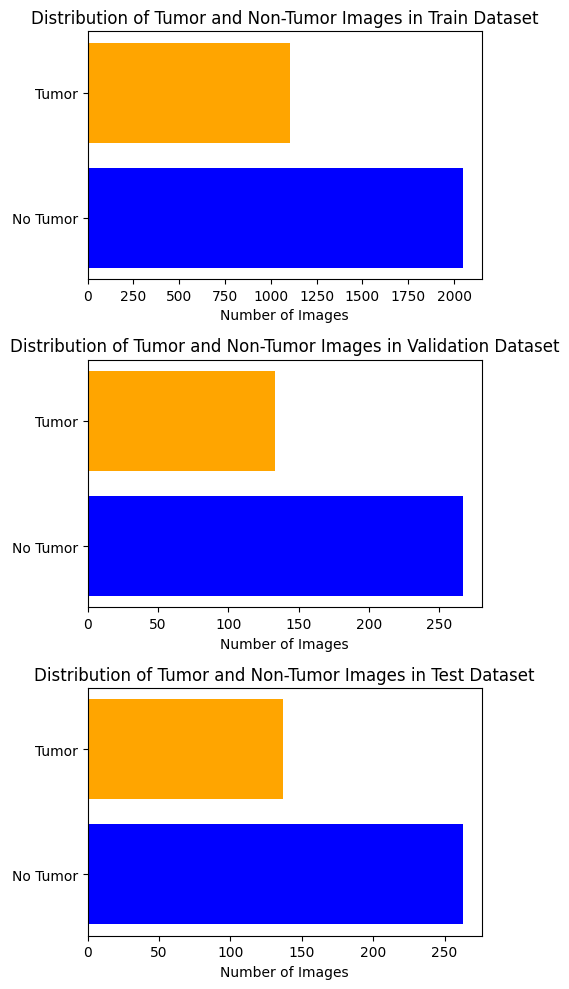
\includegraphics[width=0.75\columnwidth]{imgs/data_stats.png}
    \caption{Distributions of tumor and non-tumor images in the train, validation, and test datasets.}
    \label{fig:datastats}
\end{figure}


\section{Our Models}

Inspired by \cite{U-Mamba} and \cite{ultralightvmunet}, we sought to implement both models on a different problem: tumor segmentation.

Our goal was to 1) maintain dice scores comparable to state-of-the-art (SOTA) methods such as those listed above, while 2) being smaller than those above.

We now go into what we did for each of our models.


\subsection{UMambaBot-PP}

This model incorporates pyramidal pooling, which is a strategy used in convolutional neural networks (CNNs) to capture context and incorporate multi-scale information \cite{zhao2017pyramid}. Pyramidal pooling involves parallel pooling operations at different scales, followed by concatenation of the resulting feature maps. This approach has been shown to improve the performance of CNNs in various computer vision tasks, including segmentation, by enabling the model to capture both local and global context.

In our UMambaBot-PP model, we integrated pyramidal pooling into the U-Mamba architecture, aiming to leverage the strengths of both the Mamba module and multi-scale feature extraction.

% Unsure why this comment line is giving me troubles !!

\subsection{UL-VM-UNet-v1}
For UL-VM-UNet-v1, the initial channel list was modified from [8, 16, 24, 32, 48, 64] to [16, 32, 64, 128, 256], increasing the number of channels at each step of the encoder and decoder. Additionally, the depth of the U-Net was reduced by one layer to keep the parameter count low while increasing the number of parameters in each step. The intention was to improve performance by increasing the capacity of the model while maintaining a reasonable parameter count.

\subsection{UL-VM-UNet-v2}
In UL-VM-UNet-v2, the number of parallel branches in the Parallel Vision Mamba (PVM) block was increased from 4 to 8. This modification directly decreases the parameter count, further proving the idea proposed in the UltraLight VM-UNet paper \cite{ultralightvmunet} that processing features in parallel with reduced channel counts can significantly reduce parameters while maintaining performance. The channel list is the same as Ultra LightM-UNet's, [8,16,24,32,48,64].

\subsection{UL-VM-UNet-v3}
UL-VM-UNet-v3 combines the modifications from UL-VM-UNet-v1 and UL-VM-UNet-v2. It increases the number of parallel branches in the PVM block to 8 and modifies the channel list to [16, 32, 64, 128, 256]. Additionally, the depth of the U-Net was reduced to 5 layers. This approach aims to balance the trade-off between model capacity and parameter efficiency.

\subsection{UL-VM-UNet-v4}
This model incorporates pyramidal pooling, similar to UMambaBot-PP, but within every PVM block in both the encoder and decoder in the UltraLight VM-UNet architecture. The goal was to leverage the benefits of multi-scale feature extraction while maintaining the parameter efficiency of the UltraLight VM-UNet. Incorporating pyramidal pooling on the UL network scored slightly worse than without pyramidal pooling but required approximately 400,000 more parameters. The channel list was [16,32,64,128,256,512].

\subsection{UL-VM-UNet-v5}
UL-VM-UNet-v5 is meant to be a comparison to the -v4 and -v6 UltraLight variations. This model trained and performed well with 0.7M parameters. v5 has 8 parallels and modifies the channel list to [16,32,64,128,256,512].

\subsection{UL-VM-UNet-v6}
Another variation to further test the effects of incorporating pyramidal pooling in the UltraLight VM-UNet architecture was made by only using pyramidal pooling in the bottleneck layer, similarly done in UMambaBot-PP. The main goal here, again, was to integrate pyramidal pooling for the benefit of multi-scale feature extraction while keeping a low parameter count. The channel list was also [16,32,128,256,512].

\section{Results for Segmentation Task}
We now compare our models against ResNet18, ResNet50, standard U-Mamba bottleneck, UNet, and UltraLight VM-UNet. We train for 100 epochs on all models, and use dice-loss with Adam optimizer. We train on roughly 3000 images, and validate on roughly 400. we then test on roughly 400. We show the distributions of our data in Figure \ref{fig:datastats}.
Model results are shown in Table \ref{tab:model_comparison} and Figures \ref{fig:balls},\ref{fig:segs}.

\renewcommand{\arraystretch}{1.25}
\begin{table}[ht]
    \centering
    \captionsetup{skip=6pt}
    \begin{tabular}{|l|c|c|}
        \hline
        \textbf{Model Name} & \textbf{\#Params (M) $\downarrow$} & \textbf{Dice Score $\uparrow$} \\
        \hline
        UMambaBot-PP(Ours) & 10.0 & 0.8867 \\
        UMambaBot & 9.8 & 0.8799 \\
        ResNet18 & 13.9 & 0.8648 \\
        ResNet50 & 42.9 & 0.8672 \\
        SegFormer & 17.8 & 0.8454 \\
        UNet & \textbf{7.8} & \textbf{0.8929} \\
        \hline\hline
        UL-VM-UNet & 0.049 & 0.79955 \\
        UL-VM-UNet-v1(Ours) & 0.20 & 0.8409 \\
        UL-VM-UNet-v2(Ours) & \textbf{0.042} & 0.8243 \\
        UL-VM-UNet-v3(Ours) & 0.176 & 0.8109 \\
        UL-VM-UNet-v4(Ours) & 1.1 & 0.8548 \\
        UL-VM-UNet-v5(Ours) & 0.7 & \textbf{0.8633} \\
        UL-VM-UNet-v6(Ours) & 0.77 & 0.8628 \\
        \hline
    \end{tabular}
    \caption{Comparison of different segmentation models.}
    \label{tab:model_comparison}
\end{table}


\begin{figure}[!t]
    \centering
    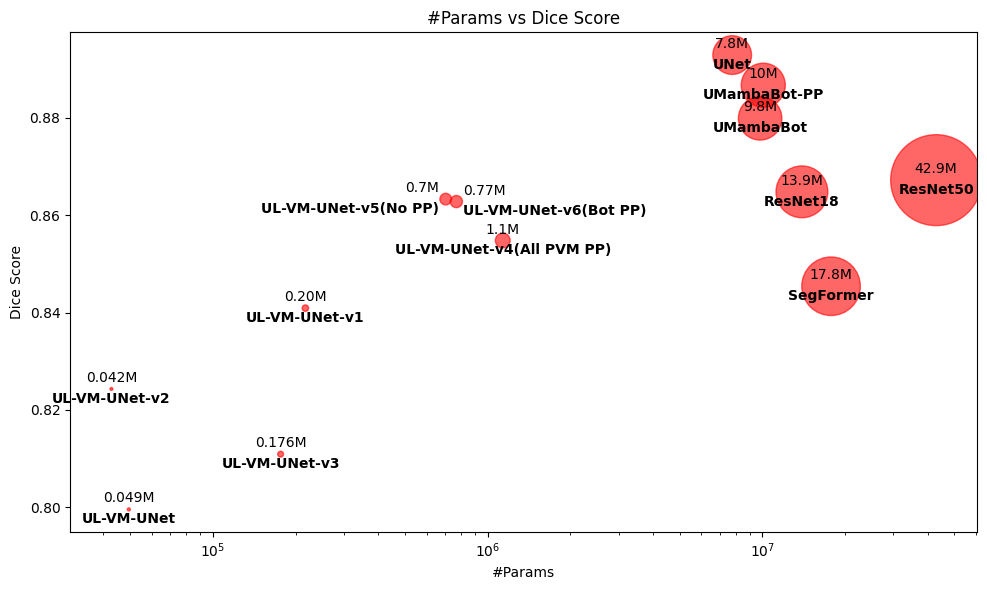
\includegraphics[width=\columnwidth]{imgs/balls.png}
    \caption{A scatter plot of Dice Score vs model parameter count, where "M" means "millions. The points are scaled to help represent size.}
    \label{fig:balls}
\end{figure}

\begin{figure}[!t]
    \centering
    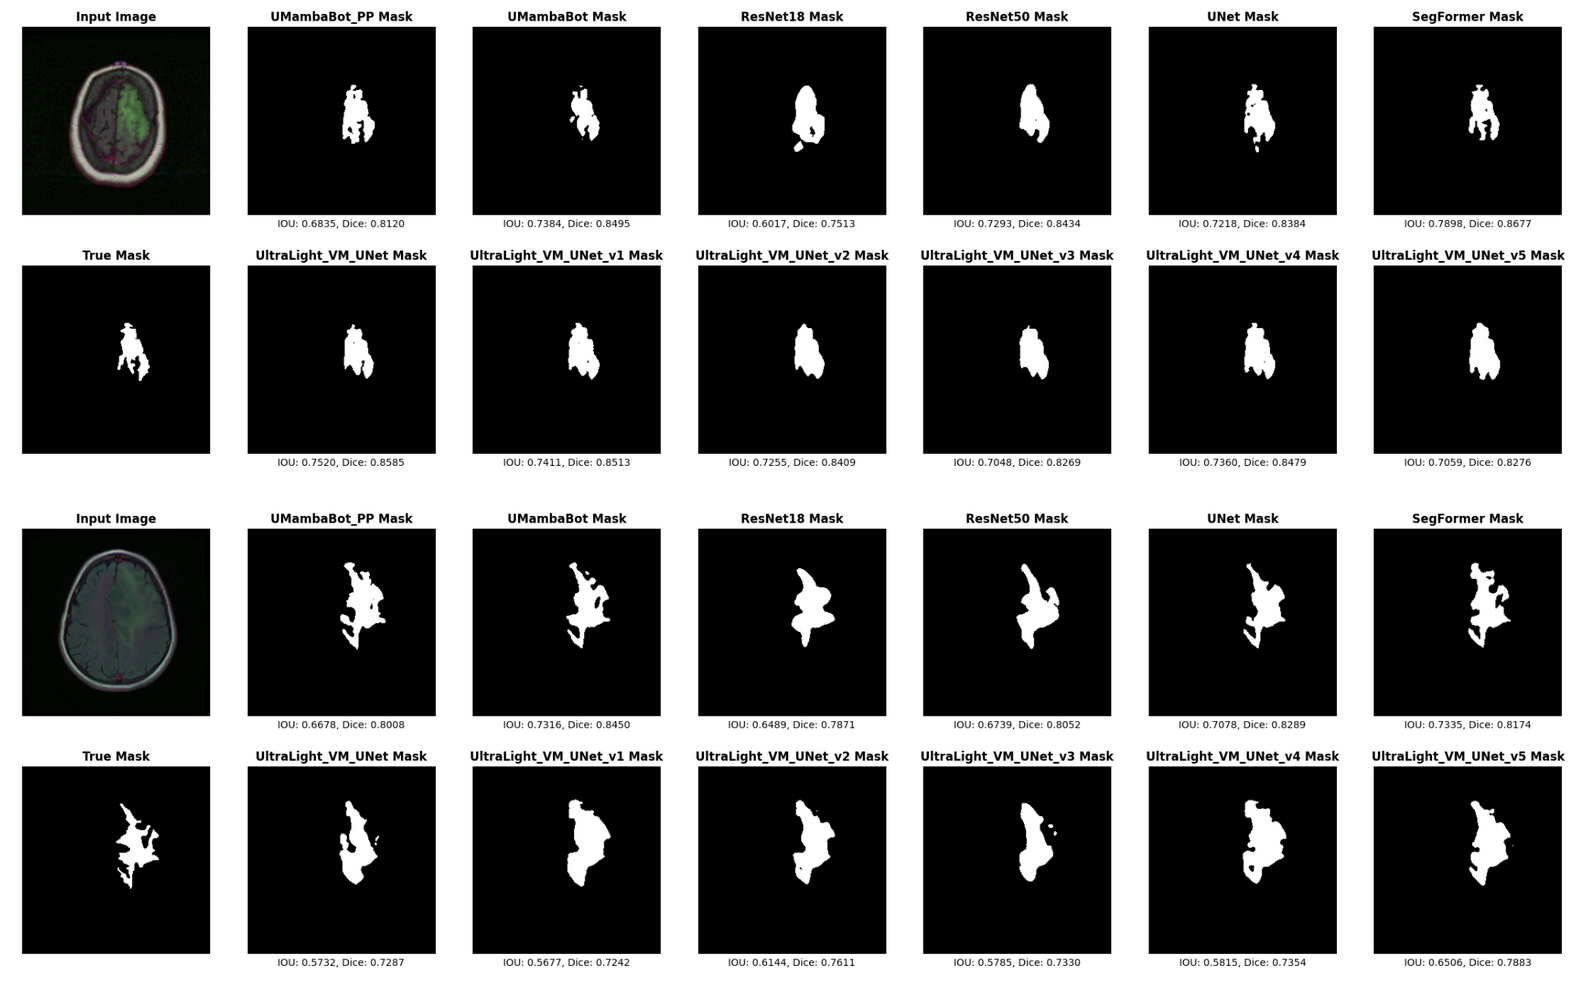
\includegraphics[width=\columnwidth]{imgs/masks.png}
    \caption{Example segmentations.}
    \label{fig:segs}
\end{figure}


\section{Application: Image Classification}
Here we investigate Mamba-based architectures with regards to the task of image segmentation.

\subsection{Input Data}\label{sec2}
To further demonstrate the viability and versatility of the Mamba architecture, we conducted experiments on the CIFAR-10 dataset \cite{krizhevsky2009learning}, a widely-used benchmark for image classification tasks. CIFAR-10 consists of 60,000 32x32 color images across 10 classes, with 6,000 images per class. The dataset is split into 50,000 training images and 10,000 test images.


\begin{figure}[!t]
    \centering
    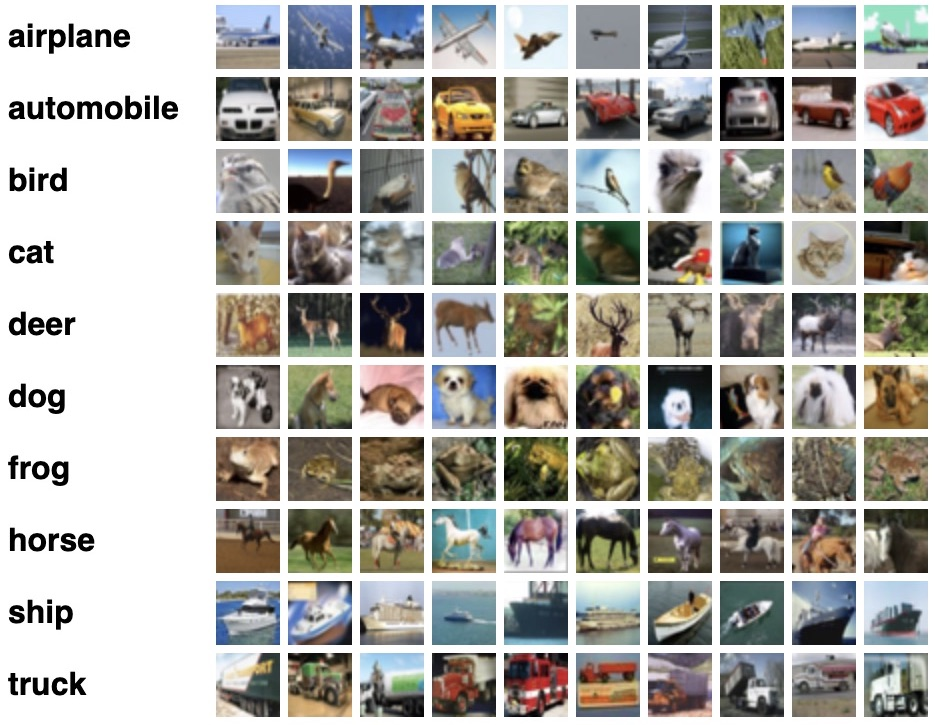
\includegraphics[width=0.75\columnwidth]{imgs/cifar_10.jpg}
    \caption{Example images from CIFAR10.}
    \label{fig:cifar}
\end{figure}


\subsection{Output Data}\label{sec3}
The output of this model will be a classification for one of the 10 classes in CIFAR10.



\section{Image Classification Models}

For this experiment, we employed the Vision Mamba (ViM) architecture proposed by Zhu et al. \cite{zhu2024vision}. ViM is an efficient visual representation learning framework that leverages a bidirectional state space model to capture long-range dependencies in visual data. By combining the strengths of CNNs and SSMs, ViM aims to achieve competitive performance while maintaining computational efficiency.

We compared the performance of ViM against the Vision Transformer (ViT) architecture \cite{dosovitskiy2021image} on the CIFAR-10 dataset. The ViM model had 1,974,664 parameters, while the ViT had 1,767,602.
Both models were trained for 100 epochs using the same experimental setup, including hyperparameters, optimization algorithm, and data augmentation techniques. Training and validation was done with batch size of 64, and upon every training iteration we do a validation iteration to obtain the validation scores. To see more on the training, please check our GitHub. The experiments were conducted on an NVIDIA GeForce RTX 3090 Ti GPU to ensure a fair comparison of training and validation times.
Figure \ref{fig:ViMViTF1} presents the validation F1 score and loss curves for both ViM and ViT over the course of 100 epochs, Figure \ref{fig:ViMViTLoss} shows the validation loss values over the 100 epochs, while Figure \ref{fig:ViMViTTrainingValidationTime} compares the training and validation times for both models. Note that ViM achieves similar performance with less training and validation time.


\section{Results for Classification Task}

These experiments demonstrate that the Mamba architecture, as implemented in the ViM model, can achieve competitive performance on image classification tasks while maintaining computational efficiency. The results highlight the potential of Mamba-based models as an alternative to transformer-based approaches, particularly in scenarios where both accuracy and efficiency are crucial considerations.


\begin{figure}[!t]
    \centering
    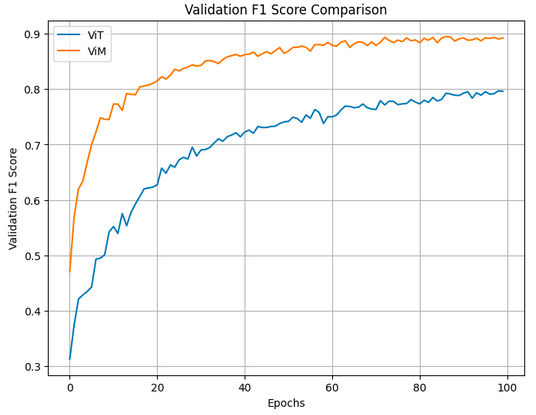
\includegraphics[width=0.75\columnwidth]{imgs/f1_comparison.png}
    \caption{F1 scores for ViM and ViT over 100 epochs.}
    \label{fig:ViMViTF1}
\end{figure}
\begin{figure}[!t]
    \centering
    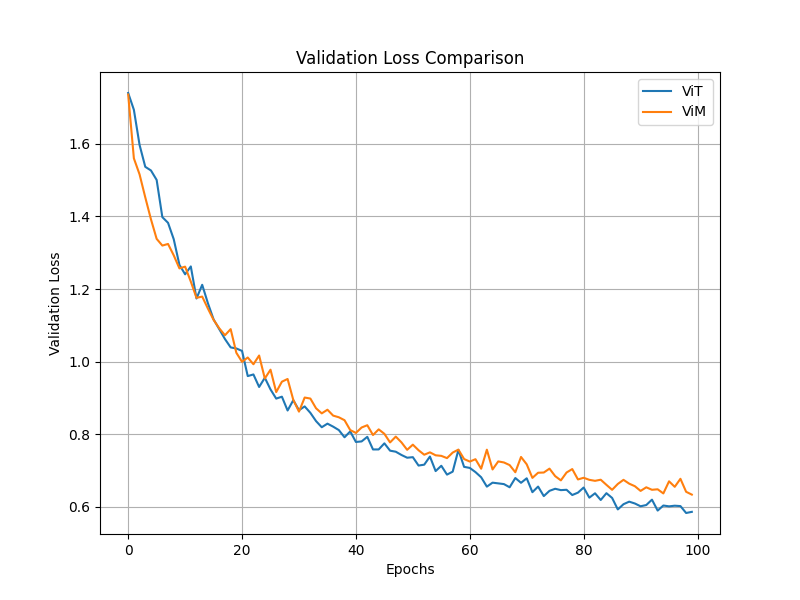
\includegraphics[width=0.75\columnwidth]{imgs/loss_comparison.png}
    \caption{Loss scores for ViM and ViT over 100 epochs.}
    \label{fig:ViMViTLoss}
\end{figure}
\begin{figure}[!t]
    \centering
    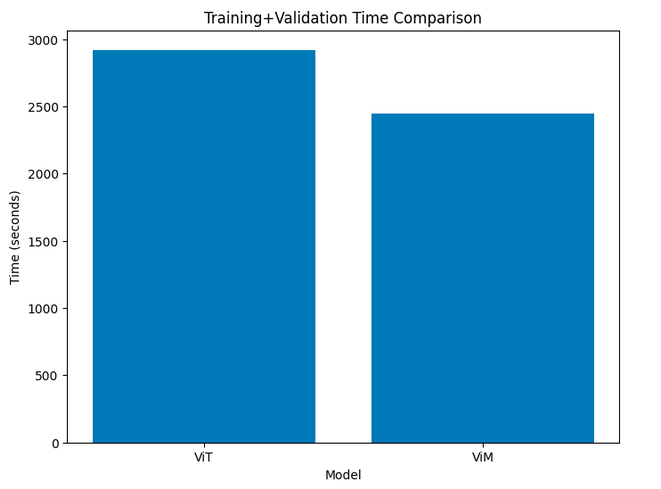
\includegraphics[width=0.75\columnwidth]{imgs/time_comparison.png}
    \caption{Training and validation time for ViT and ViM.}
    \label{fig:ViMViTTrainingValidationTime}
\end{figure}

\section{Conclusion}
We investigate the Mamba architecture with regards to the vision tasks of segmentation and classification. We develop and fine-tune models for both tasks, showing that they can outperform the SOTA in parameter count or accuracy. We hope to show that there are viable alternatives to transformers, and that 
transformer-level performance can be achieved with Mamba in the realm of computer vision.


\begin{thebibliography}{00}
    \bibitem{brown2020language} T. B. Brown et al., "Language Models are Few-Shot Learners," arXiv:2005.14165 [cs.CL], 2020.
    \bibitem{dosovitskiy2021image} A. Dosovitskiy et al., "An Image is Worth 16x16 Words: Transformers for Image Recognition at Scale," arXiv:2010.11929 [cs.CV], 2021.
    \bibitem{ronneberger2015unet} O. Ronneberger, P. Fischer, and T. Brox, "U-Net: Convolutional Networks for Biomedical Image Segmentation," arXiv:1505.04597 [cs.CV], 2015.
    \bibitem{he2016deep} K. He, X. Zhang, S. Ren, and J. Sun, "Deep Residual Learning for Image Recognition," arXiv:1512.03385 [cs.CV], 2016.
    \bibitem{vaswani2017attention} A. Vaswani et al., "Attention Is All You Need," arXiv:1706.03762 [cs.CL], 2017.
    \bibitem{gu2022efficiently} A. Gu, K. Goel, and C. Ré, "Efficiently Modeling Long Sequences with Structured State Spaces," arXiv:2111.00396 [cs.LG], 2022.
    \bibitem{simonyan2014very} K. Simonyan and A. Zisserman, “Published as a conference paper at ICLR 2015 VERY DEEP CONVOLUTIONAL NETWORKS FOR LARGE-SCALE IMAGE RECOGNITION.” Available: https://arxiv.org/pdf/1409.1556
    \bibitem{szegedy2015going} C. Szegedy et al., “Going deeper with convolutions.” Available: https://arxiv.org/pdf/1409.4842
    \bibitem{howard2017mobilenets} A. Howard et al., “MobileNets: Efficient Convolutional Neural Networks for Mobile Vision Applications.” Available: https://arxiv.org/pdf/1704.04861
    \bibitem{tan2019efficientnet} M. Tan and Q. Le, “EfficientNet: Rethinking Model Scaling for Convolutional Neural Networks.” Available: https://arxiv.org/pdf/1905.11946
    \bibitem{radosavovic2020designing} I. Radosavovic, R. Kosaraju, R. Girshick, K. He, and P. Dollár, “Designing Network Design Spaces.” Accessed: Apr. 30, 2024. [Online]. Available: https://arxiv.org/pdf/2003.13678
    \bibitem{choromanski2020rethinking} K. Choromanski et al., “Published as a conference paper at ICLR 2021 RETHINKING ATTENTION WITH PERFORMERS.” Accessed: Apr. 30, 2024. [Online]. Available: https://arxiv.org/pdf/2009.14794
    \bibitem{cheng2017survey} Y. Cheng, D. Wang, P. Zhou, and T. Zhang, “IEEE SIGNAL PROCESSING MAGAZINE, SPECIAL ISSUE ON DEEP LEARNING FOR IMAGE UNDERSTANDING 1 A Survey of Model Compression and Acceleration for Deep Neural Networks.” Accessed: Apr. 30, 2024. [Online]. Available: https://arxiv.org/pdf/1710.09282
    \bibitem{hinton2015distilling} G. Hinton, O. Vinyals, and J. Dean, “Distilling the Knowledge in a Neural Network,” 2015. Accessed: Apr. 30, 2024. [Online]. Available: https://arxiv.org/pdf/1503.02531
    \bibitem{gu2020hippo} A. Gu, T. Dao, S. Ermon, A. Rudra, and C. Ré, "HiPPO: Recurrent Memory with Optimal Polynomial Projections," Advances in Neural Information Processing Systems, vol. 33, pp. 1474-1487, 2020.
    \bibitem{vaswani2023attention} A. Vaswani et al., "Attention Is All You Need," arXiv:1706.03762 [cs.CL], 2023.
    \bibitem{gu2023mamba} A. Gu and T. Dao, "Mamba: Linear-Time Sequence Modeling with Selective State Spaces," arXiv:2312.00752 [cs.LG], 2023.
    \bibitem{U-Mamba} J. Ma, F. Li, and B. Wang, "U-Mamba: Enhancing Long-range Dependency for Biomedical Image Segmentation," arXiv:2401.04722 [cs.CV], 2024.
    \bibitem{rombach2021highresolution} R. Rombach, A. Blattmann, D. Lorenz, P. Esser, and B. Ommer, "High-Resolution Image Synthesis with Latent Diffusion Models," arXiv:2112.10752 [cs.CV], 2021.
    \bibitem{DBLP:journals/corr/abs-2006-11239} J. Ho, A. Jain, and P. Abbeel, "Denoising Diffusion Probabilistic Models," CoRR, vol. abs/2006.11239, 2020. [Online]. Available: https://arxiv.org/abs/2006.11239
    \bibitem{ultralightvmunet} R. Wu, Y. Liu, P. Liang, and Q. Chang, “UltraLight VM-UNet: Parallel Vision Mamba Significantly Reduces Parameters for Skin Lesion Segmentation.” Accessed: Apr. 20, 2024. [Online]. Available: https://arxiv.org/pdf/2403.20035.pdf
    \bibitem{zhao2017pyramid} H. Zhao, J. Shi, X. Qi, X. Wang and J. Jia, "Pyramid Scene Parsing Network," 2017 IEEE Conference on Computer Vision and Pattern Recognition (CVPR), 2017, pp. 6230-6239, doi: 10.1109/CVPR.2017.660.
    \bibitem{dataset} “Brain MRI segmentation,” www.kaggle.com. https://www.kaggle.com/datasets/mateuszbuda/lgg-mri-segmentation
    \bibitem{xie2021segformer} E. Xie, W. Wang, Z. Yu, A. Anandkumar, J. Alvarez, and P. Luo, “SegFormer: Simple and Efficient Design for Semantic Segmentation with Transformers.” Available: https://arxiv.org/pdf/2105.15203.pdf
    \bibitem{krizhevsky2009learning} A. Krizhevsky, "Learning Multiple Layers of Features from Tiny Images," Tech Report, 2009.
    \bibitem{xie2017aggregated} S. Xie, R. Girshick, P. Dollár, Z. Tu, and K. He, "Aggregated Residual Transformations for Deep Neural Networks," arXiv:1611.05431 [cs.CV], 2017.
    \bibitem{krizhevsky2012imagenet} A. Krizhevsky, I. Sutskever, and G. E. Hinton, "ImageNet Classification with Deep Convolutional Neural Networks," Advances in Neural Information Processing Systems, vol. 25, 2012.
    \bibitem{lecundocument} Y. Lecun, L. Bottou, Y. Bengio and P. Haffner, "Gradient-based learning applied to document recognition," in Proceedings of the IEEE, vol. 86, no. 11, pp. 2278-2324, Nov. 1998, doi: 10.1109/5.726791.
    \bibitem{zhu2024vision} L. Zhu, B. Liao, Q. Zhang, X. Wang, W. Liu, and X. Wang, “Vision Mamba: Efficient Visual Representation Learning with Bidirectional State Space Model,” arXiv.org, Feb. 10, 2024. https://arxiv.org/abs/2401.09417   
    \bibitem{modelSize} H. Naveed et al., “A Comprehensive Overview of Large Language Models.” Available: https://arxiv.org/pdf/2307.06435
    \bibitem{mambaNotes} U. Jamil, “hkproj/mamba-notes,” GitHub, Apr. 27, 2024. https://github.com/hkproj/mamba-notes (accessed Apr. 30, 2024).
\end{thebibliography}

\end{document}
